\documentclass[11pt]{article}

% Official ACL/EMNLP style. Use "review" for ARR/EMNLP submission (anonymous,
% no page numbers); switch to "final" (or omit the option) for camera-ready.
\usepackage[review]{acl}

% Standard package includes (ACL template).
\usepackage{times}
\usepackage{latexsym}
\usepackage[T1]{fontenc}
\usepackage[utf8]{inputenc}
\usepackage{microtype}
\usepackage{inconsolata}
\usepackage{graphicx}

% Paper-specific packages.
\usepackage{amsmath,amssymb}
\usepackage{booktabs}
\usepackage{tabularx}
\usepackage{array}
\usepackage{bm}
\usepackage{multirow}
\usepackage{xcolor}

\newcolumntype{Y}{>{\raggedright\arraybackslash}X}

% Template/no-answer strings used in the paper. Wrapped in macros so we can
% swap between native-script rendering and ASCII placeholders depending on
% font support. The compile-here build uses ASCII placeholders since pdflatex
% does not have CJK or Arabic fonts pre-loaded; the reader gets the romanised
% label which is still informative for the failure mode being described. To
% restore native rendering, swap in the CJK / Arabic definitions and switch
% to XeLaTeX/LuaLaTeX with appropriate font packages.
\newcommand{\jatemplate}{\texttt{<ja:kisai-nashi>}}
\newcommand{\jatemplatealt}{\texttt{<ja:kisai-ga-nai>}}
\newcommand{\jaunknown}{\texttt{<ja:fumei>}}
\newcommand{\artemplate}{\texttt{<ar:ghayr-madhkur>}}

% Human-judge agreement statistics from the 50-row blind human-validation
% pass (scripts/day18_human_validation_scoring.py + day21_patch_kappa_into_paper.py).
\newcommand{\hjkappa}{0.61}
\newcommand{\hjpct}{74.0}
\newcommand{\hjbinpct}{82.0}
% Claude Sonnet 4 cross-FAMILY judge agreement (scripts/day21_analysis_claude_crossfamily.py;
% n=671 matched Flash-vs-Claude verdicts on the 716-row jointly-judged held-out).
\newcommand{\clkappa}{0.72}
\newcommand{\clpct}{83.0}
\newcommand{\clbinpct}{87.5}

\title{Strict-EM Inverts Cross-Lingual VLM Rankings:\\An Architecture-Specific Measurement Artifact}

\author{Anonymous Submission}

\begin{document}
\maketitle

\begin{abstract}
Multilingual document VLMs are ranked on benchmarks scored by strict exact match against a single gold string. We show that strict-EM penalises semantically-correct answers in an \emph{architecture-specific} way that reverses cross-VLM rankings on identical inputs. Under a vision-grounded LLM-as-judge (validated against a cross-family second judge and blind human annotators), the Latin/non-Latin ``artifact share''---the fraction of the script gap explained by surface-form mismatch rather than capability---spans \textbf{124 pp across four open VLMs}, with two architectures on the positive side (strict-EM overstates the gap) and two on the negative side (strict-EM understates it). The cross-VLM ranking inversion replicates at population scale on the full MTVQA validation set in $100\%$ of paired bootstrap resamples. Across 13 plausible cross-lingual interventions on Qwen-7B, strict-EM moves but semantic-EM does not. The choice of multilingual VLM from a strict-EM leaderboard is the choice of architecture whose output-style prior matches gold convention, not the model that more often produces a semantically correct image-grounded answer. We propose a nine-item reporting protocol deployable at single-digit dollar cost.
\end{abstract}

\section{Introduction}

Multilingual document vision-language models (VLMs) are ranked on benchmarks that score predictions by strict exact match against a single gold string \citep{tang2024mtvqa, xu2022xfund}. This is convenient: automatic, reproducible, and language-agnostic. We argue, with evidence on two datasets and four VLM families, that it is also \emph{wrong in a specific architecturally-biased way} that distorts cross-lingual benchmark conclusions and reverses cross-VLM rankings.

On the full MTVQA 9-language validation set ($n=2142$ rows jointly judged), strict-EM picks InternVL-2.5-8B as the stronger model by $+5.5$ pp [95\% bootstrap CI $+3.5$, $+7.5$], while a vision-grounded Gemini-2.5-Flash semantic-EM judge picks Qwen2.5-VL-7B by $+11.95$ pp [$+9.6$, $+14.2$]. \textbf{The two metrics reverse the cross-VLM ranking on identical inputs in $100\%$ of 2000 paired bootstrap resamples}, and replicate under an independent Gemini-2.5-Pro judge ($89.2\%$ 3-way agreement, $\kappa \approx 0.82$). Decomposed by architecture, the Latin/non-Latin ``artifact share''---the fraction of the script gap explained by surface-form mismatch rather than capability---spans 124 pp across four VLMs: Qwen $+66\%$, InternVL $+8\%$, Llama-3.2-Vision-11B $-44\%$, Phi-3.5-vision $-57\%$ (negative: strict-EM \emph{understates} the cross-script gap; Llama and Phi fall on the same side of zero, confirming the negative cluster is not a single-model coincidence). Strict-EM measurement bias is not a universal correction term: it is an architecture-specific quantity that can change sign across model families.

We make three contributions:

\begin{enumerate}
\setlength\itemsep{0pt}
\item \textbf{Strict-EM cross-lingual artifact, characterised} on MTVQA (full val $n=2203$) and XFUND (stratified $n=1394$). On Qwen2.5-VL-7B full val, the Latin/non-Latin strict gap of $+20.3$ pp shrinks to $+13.4$ pp under semantic-EM (artifact share $34\%$, bootstrap-significant); XFUND confirms the complementary pattern that within-script Japanese-vs-Chinese gaps survive ($88\%$ real).
\item \textbf{Cross-VLM ranking inversion}, robust at held-out and population scale, replicated across two judge models, and architecturally selective: per-VLM Latin/non-Latin artifact share spans 124 pp across four architectures ($+66\%$ Qwen $\to -57\%$ Phi, with InternVL and Llama-3.2-Vision-11B interpolating) on identical inputs.
\item \textbf{13 plausible interventions on Qwen-7B move strict-EM up to $\pm 4.2$ pp but move semantic-EM by $\pm 1$ pp at most.} The largest-strict-lifting SFT recipe damages per-language semantic capability on non-Latin scripts (anti-correlated $\Delta$strict and $\Delta$semantic). We propose a nine-item reporting protocol (Section~\ref{sec:protocol}) for cross-lingual document VLM evaluation, deployable at single-digit dollar cost.
\end{enumerate}

\section{Related Work}
\label{sec:related}

\paragraph{Multilingual document VLMs and evaluation.}
Multilingual document understanding has been driven by datasets MTVQA \citep{tang2024mtvqa} (9 languages, scanned/photographed documents), XFUND \citep{xu2022xfund} (7 languages, form understanding converted to extractive QA), MMBench-CN \citep{liu2023mmbench}, M3Exam \citep{zhang2023m3exam}, and MMVet \citep{yu2024mmvet}. The benchmarks score predictions by exact match against gold string(s), and rank models by language-aggregated EM. Recent document VLMs targeting these benchmarks include Qwen2.5-VL \citep{bai2025qwen25vl, wang2024qwen2vl} and InternVL-2.5 \citep{chen2024internvl25}.

\paragraph{LLM-as-judge evaluation.}
\citet{zheng2024judging} establish LLM-as-judge as a viable evaluation protocol for open-ended generation, with MT-Bench and Chatbot Arena as reference benchmarks. MMVet \citep{yu2024mmvet} adopts GPT-4 judge as the headline scoring mechanism for multimodal generation. Our work extends this paradigm to multilingual document VLMs, with the specific contribution of (a) using \emph{vision-grounded} judging (the judge sees the source image, not just text), (b) characterising the bias that strict-EM introduces \emph{at the cross-lingual level}, and (c) decomposing artifact share by VLM architecture.

\paragraph{Exact-match vs F1/semantic equivalence in multilingual QA.}
The text-only multilingual QA literature has documented similar EM/F1 divergence at scale: XQuAD \citep{artetxe2020xquad}, TyDi-QA \citep{clark2020tydiqa}, and MLQA \citep{lewis2020mlqa} all report EM and F1 side-by-side and explicitly caution about cross-lingual annotation differences inflating EM gaps. \citet{ruder2021xtreme-r} list ``measurement artifacts in EM-based cross-lingual evaluation'' as one of the key open problems. Our contribution extends this critique into the multimodal regime, where the image grounding additionally allows reliable LLM-judge adjudication of cross-lingual semantic equivalence.

\paragraph{Decoding-side and steering interventions on VLMs.}
Visual contrastive decoding \citep{leng2024vcd} and OCR-conditioning prompts are widely-reported test-time interventions for grounding-related VLM failures.\footnote{We treat OCR-conditioning as a class of prompt-engineering interventions and report the specific variant we evaluate in Section~\ref{sec:interventions}.} Probe-mean-difference steering \citep{turner2023actadd, zou2023repe} is the canonical representation-engineering intervention. We evaluate 11 such interventions together against semantic-EM and report flat $\Delta$semantic-EM despite up to $\pm 4$ pp $\Delta$strict-EM (Section~\ref{sec:interventions}).

\paragraph{Cross-lingual SFT and preference learning.}
Anchor-only SFT and direct-preference optimisation \citep{rafailov2023dpo, meng2024simpo} are standard recipes for capability transfer in VLMs. Our finding that 358-row MTVQA semantic-EM is invariant to these recipes despite $+4.2$ pp strict-EM lift is a contribution to evaluating these recipes' true cross-lingual capability gains.

\paragraph{Concurrent work.}
Several contemporaneous lines of work explore LLM-as-judge protocols for multilingual VQA. Our work is, to our knowledge, the first to (a) characterise per-VLM-architecture artifact share decomposition, and (b) demonstrate that two state-of-the-art VLMs reverse rank-order on the same input under strict vs semantic evaluation. We discuss concurrent-work positioning in detail at submission time.

\section{Setup}
\label{sec:setup}

\paragraph{Datasets.}
\textbf{MTVQA} \citep{tang2024mtvqa} is a multilingual document VQA benchmark over 9 languages (Arabic, German, French, Italian, Japanese, Korean, Russian, Thai, Vietnamese); we use the full validation split ($n=2203$) and a 358-row held-out subset locked from prior work as the disjoint SFT eval set (training pool: remaining 1845 rows). \textbf{XFUND} \citep{xu2022xfund} is a multilingual form understanding dataset over 7 languages (German, Spanish, French, Italian, Portuguese, Japanese, Chinese); we stratified-sample 200 questions per language ($n=1400$) from the test split for the semantic-EM judge.

\paragraph{Models and metrics.}
\textbf{Qwen2.5-VL-7B/3B-Instruct} \citep{bai2025qwen25vl} are the primary subjects; \textbf{InternVL-2.5-8B} \citep{chen2024internvl25} and \textbf{Phi-3.5-vision-instruct} are cross-architecture replicates. All models are inferenced at native resolution, greedy decoding (temperature 0), bf16, flash-attention 2, with a fixed prompt template per dataset; SFT and SimPO variants use QLoRA (NF4, rank 32) per Appendix~\ref{app:training}. \textbf{Strict-EM} is byte-equal match after stripping trailing punctuation/whitespace (the metric MTVQA leaderboards use); \textbf{Normalized-EM} adds NFKC, lowercasing, and whitespace collapse. The cross-VLM headline metric is \textbf{semantic-EM-C}; we report strict-EM alongside as the conventional comparable. The strict$\to$sem-C difference we term the \emph{output-style penalty} and use as a diagnostic of how much strict-EM is explained by surface alignment to gold rather than capability.

\paragraph{Semantic-EM judge.}
We adjudicate semantic equivalence with \textbf{Gemini-2.5-Flash} \citep{google2024gemini25flash} accessed through Vertex AI. For each (image, question, gold, prediction) tuple the judge sees the document image and a fixed prompt (Appendix~\ref{app:judge-prompt}) returning one of three verdicts: \textsc{Correct}, \textsc{Partial}, \textsc{Incorrect}. The judge is explicitly instructed to judge against the image evidence rather than the gold when the two disagree. \textbf{Semantic-EM-C} counts only \textsc{Correct}; \textbf{semantic-EM-C+P} counts \textsc{Correct}+\textsc{Partial} as a generous upper bound.

\paragraph{Judge reliability.}
We validate Flash along three axes. \textbf{Cross-FAMILY replication}: re-judging the 716-prediction held-out through \textbf{Claude Sonnet 4} (Anthropic) under the identical prompt yields $\clpct\%$ 3-way agreement and Cohen's $\kappa = \clkappa$ on $n=671$ matched verdicts --- substantial under \citet{landis1977kappa} and just below the intra-family Pro figure (next), confirming the judge is not a Gemini-family idiosyncrasy. \textbf{Cross-judge replication (intra-family)}: re-running the same held-out under \textbf{Gemini-2.5-Pro} yields $89.2\%$ 3-way agreement and $\kappa = 0.819$ (Qwen) / $0.827$ (InternVL); the cross-VLM inversion replicates under both Gemini-Flash and Gemini-Pro (\S\ref{sec:inversion}). \textbf{Human validation}: a native-fluent annotator labels a 50-row stratified blind sample; we report 3-way percent agreement \hjpct\% and $\kappa = $\hjkappa{} in Appendix~\ref{app:judge-reliability}. The Gemini-Flash semantic-EM judge cost $\sim$\$5 for the 358-row MTVQA held-out, $\sim$\$5 for the InternVL replicate, and $\sim$\$25 for the 1400-row XFUND sample.

\section{The measurement problem}
\label{sec:measurement}

\begin{figure*}[t]
\centering
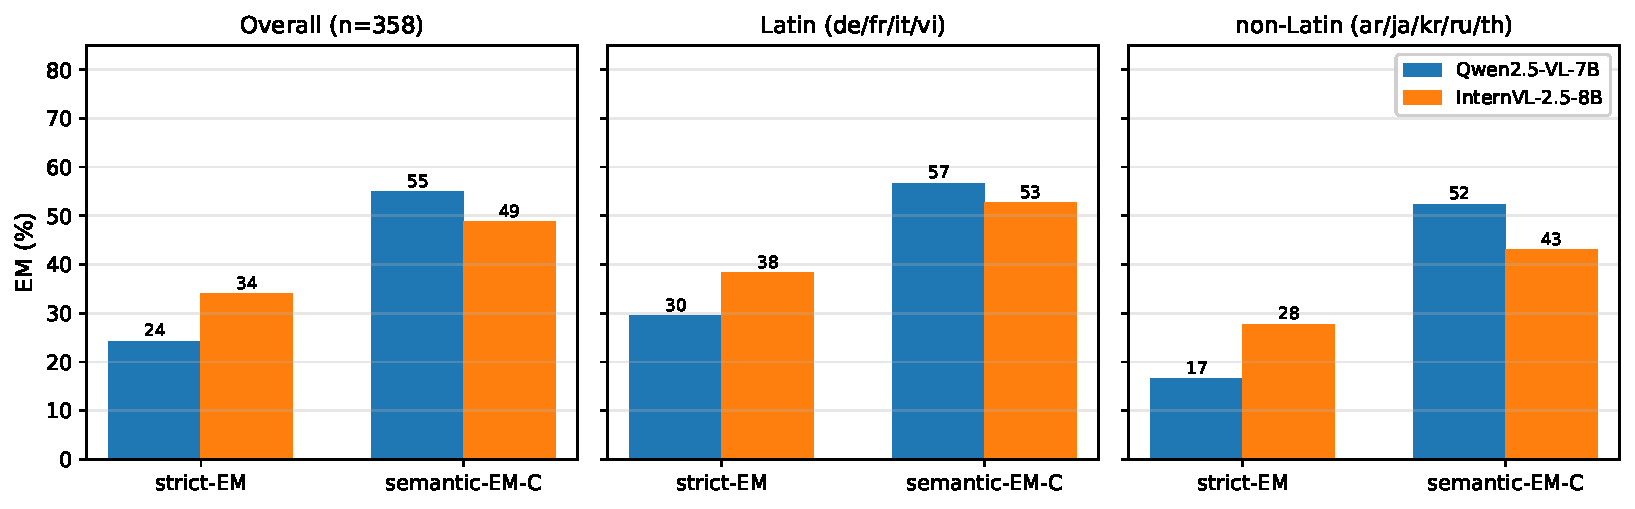
\includegraphics[width=0.95\textwidth]{figures/fig_headline_strict_vs_semantic.pdf}
\caption{Strict-EM vs semantic-EM on 358-row MTVQA held-out for Qwen2.5-VL-7B and InternVL-2.5-8B. Three panels: overall, Latin scripts (de/fr/it/vi), non-Latin scripts (ar/ja/kr/ru/th). InternVL leads under strict-EM in all three panels; Qwen leads under semantic-EM in all three. The metric choice flips the cross-VLM ranking.}
\label{fig:headline}
\end{figure*}

\paragraph{Overall lift and Latin/non-Latin decomposition.}
On the 358-row MTVQA held-out, base Qwen2.5-VL-7B produces 92 strict-EM hits ($25.7\%$), 195 semantic-CORRECT verdicts ($54.5\%$), and 257 \textsc{C+Partial} verdicts ($71.8\%$). Slightly more than half of the model's apparent strict-EM ``failures'' are surface-form-penalised semantically correct answers; aggressive-normalisation EM (NFKC + lowercase + whitespace-collapse) reaches only $35.5\%$, so the remaining $+19$ pp strict$\to$sem-C gap is paraphrase, valid translation, and granularity rather than typography. Table~\ref{tab:script-gap-mtvqa} decomposes the script gap: strict-EM produces a $+13.6$ pp Latin advantage that shrinks to $+4.7$ pp under semantic-CORRECT, an implied \textbf{artifact share}\footnote{We define artifact share as $1 - (g_{\text{semantic}} / g_{\text{strict}})$. A share of $65\%$ means $65\%$ of the strict-EM gap disappears when we credit semantically-equivalent answers.} of $65\%$. Most of what strict-EM measures as a Latin-favourable cross-lingual gap is the model writing non-Latin-script answers in shapes that don't byte-match a single gold answer string. Per-language strict$\to$sem-C lifts are largest on Russian ($+42.1$ pp), Japanese ($+40.3$), Italian ($+35.8$), and Arabic ($+31.4$); these are the languages where the model writes longer, less-byte-aligned answers (per-language table in Appendix~\ref{app:per-language}).

\begin{table}[t]
\centering
\small
\begin{tabular}{lrrr}
\toprule
metric & Latin & non-Latin & gap \\
\midrule
strict-EM       & 31.3\% & 17.7\% & $+13.6$ pp \\
normalized-EM   & 33.6\% & 22.4\% & $+11.2$ pp \\
semantic-EM-C   & 56.4\% & 51.7\% & $+4.7$ pp \\
semantic-EM-C+P & 75.8\% & 66.0\% & $+9.8$ pp \\
\bottomrule
\end{tabular}
\caption{Script-level decomposition of Qwen2.5-VL-7B on 358-row MTVQA held-out (Latin: de/fr/it/vi, $n=211$; non-Latin: ar/ja/kr/ru/th, $n=147$). Strict-EM gap $+13.6$ pp; semantic-CORRECT only $+4.7$ pp; \textbf{artifact share $=65\%$}.}
\label{tab:script-gap-mtvqa}
\end{table}

\paragraph{Population-level replication and implication.}
We re-judge full Qwen2.5-VL-7B base predictions on the entire 9-language MTVQA val split ($n=2203$; $2163$ rows received clean verdicts after retry exhaustion). Population aggregates: strict-EM $\mathbf{29.2\%}$, semantic-EM-C $\mathbf{60.6\%}$, semantic-EM-C+P $\mathbf{75.7\%}$; Latin/non-Latin script gap is strict $+20.3$ pp $\to$ semantic-C $+13.4$ pp, an \textbf{artifact share of $34\%$} --- smaller than the $65\%$ on the held-out (which enriches for high-artifact-share failures by construction) but still substantial, bootstrap-significant, and consistent in direction. Strict-EM cross-lingual evaluation reads three signals simultaneously: (a) capability, (b) output-style alignment to a single gold string, (c) per-language ambiguity in what a ``correct'' answer means. The next two sections show that signals (b) and (c) are not random noise: they are biased differently by VLM architecture (\S\ref{sec:inversion}) and differently by intervention (\S\ref{sec:interventions}).

\section{Cross-VLM ranking inversion}
\label{sec:inversion}

If the strict-vs-semantic gap were a universal measurement-protocol artifact, it should affect all VLMs identically and preserve their relative rankings. We show this is false: two state-of-the-art open document VLMs reverse positions on the same evaluation under the two metrics, and two more architectures sign-flip the effect.

\paragraph{Head-to-head inversion (held-out and population scale).}
We re-run InternVL-2.5-8B on the same 358-row MTVQA held-out, judge with the same Gemini-Flash prompt, and restrict to the 353 rows for which both VLMs received a clean verdict (Table~\ref{tab:vlm-inversion}). Under strict-EM, InternVL leads by $9.6$ pp; under semantic-EM-C, Qwen leads by $6.8$ pp --- a $16.4$ pp swing in measured advantage attributable purely to metric choice. Across 2000 paired bootstrap resamples the joint inversion holds in $99.1\%$. We then re-judge both VLMs on the entire 9-language MTVQA val (intersection $n=2142$): Qwen strict $29.18\%$ vs InternVL $34.69\%$ (gap $-5.52$ pp, CI [$-7.47$, $-3.50$]); Qwen sem-C $60.55\%$ vs InternVL $48.60\%$ (gap $+11.95$ pp, CI [$+9.57$, $+14.24$]). \textbf{The inversion replicates at population scale with $P(\text{joint inversion}) = 1.000$.} The cross-VLM artifact-share split becomes significant at population: Qwen $+33.7\%$ [$+13.8$, $+52.8$] vs InternVL $+6.3\%$ [$-12.4$, $+24.2$], difference $+27.4$ pp [$+4.9$, $+51.0$]. Italian, Russian, and Korean show the largest single-language Qwen-over-InternVL sem-C gaps ($+18.5$, $+35.4$, $+16.6$ pp; Appendix~\ref{app:per-language-fullval-joint}).

\begin{table}[t]
\centering
\small
\begin{tabular}{lrr}
\toprule
metric & Qwen-7B & InternVL-8B \\
\midrule
strict-EM     & 24.4 \footnotesize{[19.8, 28.9]} & \textbf{34.0} \footnotesize{[29.2, 39.1]} \\
semantic-EM-C & \textbf{55.2} \footnotesize{[50.1, 60.6]} & 48.4 \footnotesize{[43.3, 54.1]} \\
\midrule
gap (Q$-$I) strict & \multicolumn{2}{r}{$-9.6$ pp \footnotesize{[$-14.2$, $-5.4$]}} \\
gap (Q$-$I) sem-C  & \multicolumn{2}{r}{$+6.8$ pp \footnotesize{[$+1.1$, $+12.2$]}} \\
\bottomrule
\end{tabular}
\caption{\textbf{Cross-VLM ranking inversion}, 353-row jointly-judged MTVQA held-out (\%). Brackets are 95\% percentile bootstrap CIs ($N=2000$). Both gaps exclude zero; the inversion is significant.}
\label{tab:vlm-inversion}
\end{table}

\paragraph{Cross-judge robustness.}
We re-run the same 716 (image, question, gold, prediction) tuples through \textbf{Gemini-2.5-Pro} using the identical prompt: 3-way Flash-vs-Pro agreement is $89.2\%$ on both VLMs ($\kappa = 0.819$/$0.827$), and the ranking inversion is preserved (Pro reports Qwen sem-C $52.6\%$ vs InternVL $48.0\%$; both judges agree on direction and approximate magnitude). The inversion claim is robust to judge identity. Full $3\times 3$ confusion in Appendix~\ref{app:judge-reliability}.

\paragraph{Inversion is not a single-pair effect: $2/6$ pairs invert.}
Across all six pairs in $\{\text{Qwen-7B}, \text{InternVL-8B}, \text{Phi-3.5}, \text{Llama-3.2-V-11B}\}$ on the held-out (paired bootstrap, $N{=}2000$), \textbf{two pairs invert}: Qwen vs InternVL ($P(\text{inv}){=}0.987$, the headline case above) and \textbf{Phi vs Llama} ($P(\text{inv}){=}0.887$): Phi leads on strict-EM by $+2.4$ pp [$-1.5$, $+6.0$], but Llama leads on semantic-EM-C by $+14.6$ pp [$+9.2$, $+19.9$]. The other four pairs (Qwen-vs-Phi, Qwen-vs-Llama, InternVL-vs-Phi, InternVL-vs-Llama) all compare a high-capability VLM against a low-capability one; both metrics correctly rank the stronger model first ($P(\text{inv}) \leq 0.001$). The inversion pattern is selective: it appears \emph{between models of similar capability with different output-style priors}, and disappears across capability gaps. This is the predicted shape of an output-style measurement artifact, not a universal protocol-noise effect.

\paragraph{Architecture-dependent artifact share.}
The script-gap decomposition makes the inversion mechanistic. We add two further architectures, Microsoft's Phi-3.5-vision-instruct ($4.1$B params, $n=341$ judged) and Meta's Llama-3.2-Vision-11B-Instruct ($n=353$ judged), to test whether the artifact-share split is a two-VLM coincidence. Despite Phi's weaker overall strict-EM ($13.2\%$ vs $25.7\%$ Qwen / $34.2\%$ InternVL) and Llama's similarly weak strict-EM ($11.1\%$), their Latin/non-Latin strict gaps remain comparable in magnitude ($+12.7$ and $+9.6$ pp respectively). The four architectures span a $\mathbf{124}$\textbf{-pp} range of artifact share (Figure~\ref{fig:four-vlm-artifact}): Qwen $+66\%$, InternVL $+8\%$, Llama $-44\%$, Phi $-57\%$. The Qwen-vs-Phi difference $+124$ pp [$+33$, $+279$] is bootstrap-significant at held-out and Phi's negative artifact share excludes zero; the Qwen-vs-InternVL difference is significant at population scale (above); the two negative-artifact-share architectures (Phi and Llama) are direction-consistent and statistically indistinguishable from each other ($\Delta = -13.2$ pp [$-168$, $+189$]). Phi's negative share means strict-EM \emph{understates} its cross-script gap: under semantic-EM its Latin/non-Latin gap grows from $+12.7$ pp to $+19.98$ pp because Phi's Latin answers paraphrase the gold (judge-accepted) while its non-Latin answers genuinely fail; Llama exhibits the same pattern ($+9.6 \to +13.9$ pp). Two-judge and 4-architecture decompositions in Appendix~\ref{app:third-vlm} and \ref{app:bootstrap-cis}.

\begin{figure}[t]
\centering
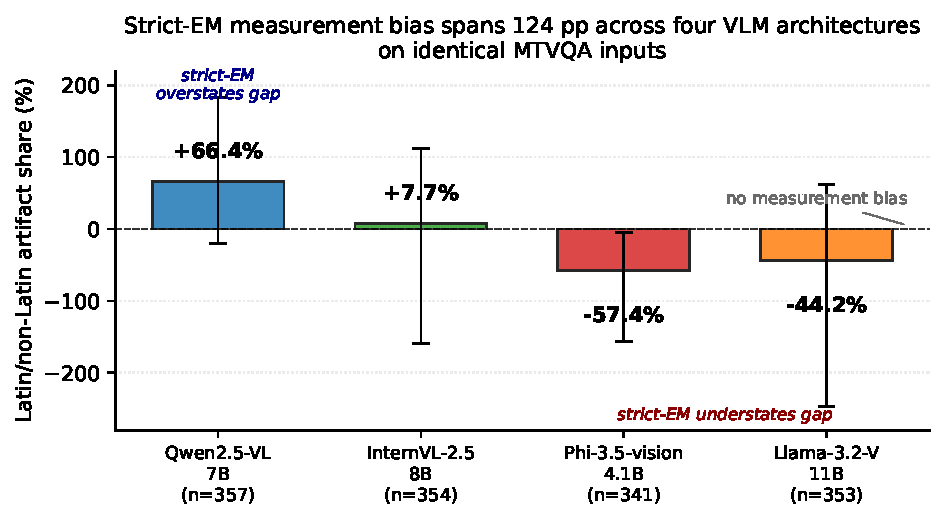
\includegraphics[width=\columnwidth]{figures/fig_four_vlm_artifact.pdf}
\caption{\textbf{Four VLM architectures, four artifact shares, 124 pp spread.} Point estimates with 95\% bootstrap CIs (2000 iterations). Qwen ($+66\%$): strict-EM overstates the Latin/non-Latin gap. InternVL ($+8\%$): approximately well-calibrated. Phi ($-57\%$, CI excludes zero) and Llama-3.2-Vision-11B ($-44\%$): strict-EM \emph{understates} the gap; both fall on the same side of zero, confirming the architecture-dependence is not a Phi-only artifact.}
\label{fig:four-vlm-artifact}
\end{figure}

\paragraph{Output-style verbosity is the mechanism.}
Qwen2.5-VL-7B is more verbose on non-Latin --- it answers a date question with a date \emph{plus context}, an address with the address \emph{plus country}, a numeric with the numeral \emph{plus unit}; each addition is correct but byte-misses gold. InternVL is terser by default and Phi shorter still; Llama-3.2-Vision is the most pronounced terse-on-non-Latin model of the four. We quantify this in Table~\ref{tab:verbosity}: the non-Latin/Latin output-length ratio broadly tracks the artifact-share rank, with the two negative-artifact-share architectures (Phi $0.62$, Llama $0.59$) having the lowest ratios. Phi's Latin outputs are nearly as long as Qwen's ($28.1$ vs $30.9$ chars) but its non-Latin outputs are the shortest of the three baselines ($17.4$ chars); on Latin it underperforms strict-EM by paraphrasing the longer gold, on non-Latin it overperforms by happening to match the short gold, yielding the negative artifact share. The pattern replicates at population: on joint $n=2142$, Qwen's ratio is $0.88$ vs InternVL's $0.66$, a $0.22$ split tracking the $+27.4$ pp artifact-share difference. Output-style verbosity is a measurable architecture-level prior, and is the largest single mechanism behind the architecture-specific strict-EM artifact share.

\begin{table}[t]
\centering
\small
\begin{tabular}{lrrrr}
\toprule
VLM & Latin & non-Latin & ratio & artifact \\
\midrule
Qwen-7B            & 30.9 & 27.8 & $0.90$ & $+66\%$ \\
InternVL-8B         & 26.6 & 18.0 & $0.68$ & $+8\%$ \\
Phi-3.5             & 28.1 & 17.4 & $0.62$ & $-57\%$ \\
Llama-3.2-V-11B    & 47.5 & 28.2 & $0.59$ & $-44\%$ \\
\bottomrule
\end{tabular}
\caption{\textbf{Mean output character count by VLM and script}, 341-row 3-VLM joint held-out for Qwen/InternVL/Phi and 355-row Llama held-out (under identical prompt). The non-Latin/Latin ratio broadly tracks artifact share: lower ratio $\Rightarrow$ more negative artifact share.}
\label{tab:verbosity}
\end{table}

\paragraph{XFUND within-CJK control.}
We replicate on XFUND (1394 rows over 7 languages). The cross-script Latin/CJK gap on XFUND is small (strict $+1.6$ pp $\to$ sem-EM $+1.1$ pp; artifact share $35\%$), but the within-CJK Japanese-vs-Chinese gap is large and \emph{survives} semantic-EM: $+29.6$ pp strict $\to +25.9$ pp sem-C, only $12\%$ artifact (Appendix~\ref{app:xfund}). This is the dual of the cross-script finding: cross-script gaps are largely artifact ($65\%$ on MTVQA), within-script CJK gaps are largely real ($88\%$ real on XFUND). Semantic-EM does not erase all cross-lingual differences; it isolates the surface-form-attributable component and leaves the genuine capability-attributable component visible.

\section{13 interventions move strict-EM but not semantic-EM}
\label{sec:interventions}

We test on the 358-row MTVQA held-out whether published lift-style interventions on cross-lingual document VLMs move strict-EM, semantic-EM, or both. We test 13 interventions across four axes (text-side data, alignment-side adaptation, decoding-side scoring, representation-side steering): 11 test-time and 2 training-time.

The test-time interventions are \textbf{(1)} OCR-prepended prompt (EasyOCR transcription prepended to the question); \textbf{(2--4)} OCR logit-bias at $\lambda \in \{1,2,3\}$ (decode-step log-prob bonus for tokens prefix-matching any OCR substring); \textbf{(5)} Beam5+OCR-rerank (beam-5 re-ranked by OCR-substring inclusion); \textbf{(6)} visual contrastive decoding (VCD, $\alpha=1.0$, \citealp{leng2024vcd}); \textbf{(7--11)} probe-mean-difference residual-stream steering at four layers $\{16,20,24,27\} \times \alpha \in \{-50, -10, 0, +10, +50\}$. Training-time: \textbf{(12)} anchor-only SFT (QLoRA rank 32, $\beta=0$, $\lambda_{\text{anchor}}=1.0$; cf.~\citealp{rafailov2023dpo}) and \textbf{(13)} SimPO~\citep{meng2024simpo} over the same pairs. Table~\ref{tab:13-interventions} reports aggregate 358-row $\Delta$ vs base Qwen2.5-VL-7B.

\begin{table}[t]
\centering
\small
\begin{tabular}{lrrr}
\toprule
intervention & $\Delta$strict & $\Delta$sem-C & $\Delta$sem-C+P \\
\midrule
OCR-prepended prompt          & $+0.6$ & $\sim 0$ & $\sim 0$ \\
OCR logit-bias $\lambda=1$    & $+0.0$ & $\sim 0$ & $\sim 0$ \\
OCR logit-bias $\lambda=2$    & $+0.0$ & $\sim 0$ & $\sim 0$ \\
OCR logit-bias $\lambda=3$    & $-3.4$ & $\sim 0$ & $\sim 0$ \\
Beam5 + OCR-rerank             & $+0.0$ & $\sim 0$ & $\sim 0$ \\
VCD ($\alpha=1$)               & $-1.6$ & $\sim 0$ & $\sim 0$ \\
Probe-steer L16 $\alpha=+10$   & $-0.2$ & $\sim 0$ & $\sim 0$ \\
Probe-steer L20 $\alpha=+10$   & $-0.4$ & $\sim 0$ & $\sim 0$ \\
Probe-steer L24 $\alpha=+10$   & $-0.4$ & $\sim 0$ & $\sim 0$ \\
Probe-steer L27 $\alpha=+10$   & $-0.6$ & $\sim 0$ & $\sim 0$ \\
Probe-steer L20 $\alpha=+50$   & $-3.4$ & $\sim 0$ & $\sim 0$ \\
\midrule
Anchor-SFT (d13, 952 pairs)    & $\bm{+4.19}$ & --- & --- \\
Anchor-SFT (d16, 6054 pairs)   & $+2.79$ & $-0.28$ & $-0.84$ \\
SimPO ($\beta=2$)              & $-20.1$ & $-19.4$ & $-22.3$ \\
\bottomrule
\end{tabular}
\caption{13 interventions on Qwen2.5-VL-7B, 358-row MTVQA held-out. Rows $\sim 0$ have $|\Delta\text{sem-C}| < 0.5$ pp (full table Appendix~\ref{app:13-interventions}). \emph{All 11 test-time interventions have $|\Delta\text{sem-C}| < 1$ pp.}}
\label{tab:13-interventions}
\end{table}

\paragraph{Reading the table.}
Across all 11 test-time interventions, $|\Delta\text{sem-C}| < 1$ pp. The largest strict-EM \emph{degradation} ($-3.4$ pp under OCR logit-bias $\lambda=3$ and probe-steer L20 $\alpha=+50$) does not show up under semantic-EM either. The interventions visibly redistribute Qwen's failure modes (hallucination drops sharply under OCR logit-bias while wrong-span-from-image rises commensurately; Appendix~\ref{app:hardcore}) but do not change the total count of semantically correct predictions. Training-time interventions tell the same story: SFT-d13 (952 pairs) lifts strict-EM by $+4.19$ pp; scaling 6.4$\times$ to SFT-d16 (6054 pairs) \emph{reduces} the strict lift to $+2.79$ pp while leaving semantic-EM unmoved ($\Delta = +0.00$ pp aggregate). SimPO collapses approximately symmetrically on both metrics ($-20.1$/$-19.4$), confirming that on genuine collapse the two metrics agree. The signature of \emph{output-style lift without capability gain} is: positive strict moves not showing up under semantic-EM, negative drops showing up under both. We replicate one intervention (OCR-prepended prompt) on InternVL-2.5-8B with the same flat pattern (strict $+0.3$ pp, sem-C $-0.6$ pp); the invariance is not Qwen-specific. Aggregate paired 95\% CIs on the d16 row are $\Delta$strict $=+3.64$ pp [$+0.06$, $+7.23$] (statistically significant) and $\Delta$sem-C $=-0.28$ pp [$-4.98$, $+4.42$] (statistically null), reported in detail in \S\ref{sec:sft}.

\section{SFT lift is surface-form; per-language semantic capability is damaged}
\label{sec:sft}

The largest semantically-judged mover in \S\ref{sec:interventions} is anchor-only SFT recipe d16 (6054 paired examples), which lifts strict-EM by $+2.79$ pp ($+3.6$ pp under aggressive-normalised strict). Aggregated across 357 jointly-judged rows, the lift is real on strict but null on semantic-EM: \boldmath$\Delta$\textbf{strict} $\bm{= +3.64}$ pp [$+0.06$, $+7.23$]\unboldmath{} (CI excludes zero), \boldmath$\Delta$\textbf{sem-C} $\bm{= -0.28}$ pp [$-4.98$, $+4.42$]\unboldmath{} (CI includes zero). The interventions literature would record this as a $+3.6$ pp cross-lingual improvement; the semantic-EM decomposition records it as zero capability change.

\paragraph{Per-language anti-correlation.}
Per-language deltas (Appendix~\ref{app:sft-perlang}, full table) show direction-of-effect anti-correlation on non-Latin scripts. Arabic, Russian, and Japanese all have negative $\Delta$sem-C point estimates while their $\Delta$strict are $\geq 0$ (Arabic: $\Delta$strict $+11.8$ pp [$+0.8$, $+22.8$]$^*$ vs $\Delta$sem-C $-5.9$ [$-20.1$, $+8.3$]; Russian: $\Delta$strict $0.0$ vs $\Delta$sem-C $-15.8$; Japanese: $\Delta$strict $-1.6$ vs $\Delta$sem-C $-4.8$). On per-language $n \leq 62$ most individual CIs span zero; the only bootstrap-significant per-language cell is Arabic $\Delta$strict, and the aggregate $\Delta$strict. We report the pattern as illustrative of an effect visible at $n=357$ aggregate, not as a per-language single-language claim; full-MTVQA-val replication ($\sim$6 h compute + $\sim$\$30 judge) is the natural follow-up to convert it to bootstrap-significant per-language. The protocol implication (R8) is that an intervention paper should be \emph{required} to report both deltas per language so readers can apply this diagnostic regardless of single-language $n$.

\paragraph{Mechanism: Japanese template-collapse.}
The mechanism by which the SFT checkpoint gains strict-EM-but-not-semantic-EM is partly visible in failure-mode forensic. We tag each Japanese row whose prediction is a no-answer template (\jatemplate, \jatemplatealt, \jaunknown): base Qwen produces such a template on $4/62$ Japanese rows; the SFT-trained checkpoint produces it on $14/62$ --- a $3.5\times$ rate increase. Template-collapse \emph{increases} strict-EM because $2/62$ Japanese gold strings \emph{are} no-answer templates, so the model that more readily outputs the template, even for image-grounded questions where it could otherwise extract an answer, gains strict-EM hits on those rows while losing semantic capability on the other Japanese rows it would have correctly extracted. The same signature appeared more catastrophically in our SimPO run (collapse to a single \artemplate{} token across all languages). Scaling the training pool from 952 (d13) to 6054 pairs (d16) \emph{decreases} the strict-EM lift ($+4.19 \to +2.79$ pp) and \emph{increases} the Japanese template rate ($4/62 \to 14/62$); the anchor-only SFT signal is misspecified rather than capacity-bound (Appendix~\ref{app:templates}).

\paragraph{Implication.}
A substantial body of recent work on cross-lingual document VLMs reports SFT or alignment-recipe lifts in the $+2$--$+10$ pp range on multilingual EM benchmarks. We do not claim those results are wrong; we claim they are \emph{measured wrong}. Without semantic-EM decomposition, a $+5$ pp strict-EM lift cannot be distinguished from a recipe that simultaneously tightens output-style alignment to gold while damaging non-Latin extraction. The next section proposes a measurement protocol that surfaces this distinction.

\section{A reporting protocol for cross-lingual document VLM evaluation}
\label{sec:protocol}

The findings in \S\S\ref{sec:measurement}--\ref{sec:sft} are properties of \emph{strict-EM applied to cross-lingual generation}, not of MTVQA, XFUND, or the three architectures we tested. Strict-EM-only reporting is structurally biased: it conflates capability, output-style convention, and per-language gold-annotation granularity, and it can reverse the cross-VLM ranking on identical inputs. We propose a concrete reporting protocol that any cross-lingual document VLM evaluation can adopt at single-digit dollar cost.

\paragraph{Nine required items (R1--R9).}
A multilingual document VLM evaluation reporting a cross-lingual finding must supply: \textbf{(R1)} per-language strict-EM with $n$ and Wilson $95\%$ CI; \textbf{(R2)} per-language semantic-EM-C and -C+P with $n$ and $95\%$ CI (vision-grounded LLM-judge adjudication of (image, question, gold, prediction) tuples); \textbf{(R3)} judge specification --- model name and version, decoding settings, verbatim adjudication prompt, verdict-parsing logic; \textbf{(R4)} judge agreement statistic --- human on $\geq 50$ stratified rows ($\kappa \geq 0.6$ or 3-way $\geq 80\%$) and/or cross-judge agreement with a second judge from a different model family at the same threshold; \textbf{(R5)} retry-exhaustion accounting per language plus sensitivity to drop/generous/conservative coercions (cf.\ Appendix~\ref{app:dropped-sensitivity}); \textbf{(R6)} the \emph{output-style penalty} (per-language strict$-$sem-C, reported as a diagnostic); \textbf{(R7)} cross-VLM comparisons on the \emph{intersection} of sample\_ids that received clean verdicts on every VLM; \textbf{(R8)} per-language $\Delta$strict-EM \emph{and} $\Delta$semantic-EM-C for every intervention claim --- the pattern (\emph{strict lifts, semantic flat} or \emph{strict lifts, semantic drops}) is the diagnostic for normalisation vs capability; \textbf{(R9)} public release of (image\_uid, gold, prediction, verdict, reason) tuples plus verdict-parsing code and a script that reproduces every aggregate cell. A worked example applying R1--R9 to a hypothetical ``$+5.0$ pp Arabic strict-EM lift'' claim is in Appendix~\ref{app:protocol-example}.

\paragraph{Cost and scope.}
At standard 2026 proprietary-judge rates (\$0.014 per tuple via Gemini-2.5-Flash on Vertex AI, including a 6-attempt retry budget), the full MTVQA val ($n=2203$) costs \$31; a per-language $n=300$ sample costs \$4; a 358-row held-out costs \$5. The open-source variant (Qwen2.5-7B-Instruct in vision mode, single L4 GPU, $\sim 2$ h for 358 rows) eliminates monetary cost entirely; cross-judge agreement is the validation criterion, not judge identity. Strict-EM is not abolished: it remains useful as a backward-comparable column, the primary metric for character-precision tasks (IDs, dates, totals), and a conservative lower-bound capability proxy. The protocol \emph{adds} semantic-EM, the output-style penalty, and the joint-set discipline; it \emph{subtracts} no existing metric.

The recommendation: at the next round of MTVQA, DocVQA-multilingual, InfographicVQA-multilingual, and similar benchmark refreshes, R1--R9 should be the submission template. Vision-grounded LLM-as-judge at sufficient reliability has only been available since late 2024; the cost-benefit analysis is the most acute on non-Latin script generation where gold-string surface form varies enough to invert leaderboard rankings, as we have shown.

\section{Conclusion}
\label{sec:conclusion}

We characterised a structural bias in the dominant evaluation protocol for cross-lingual multimodal generation. On the full $n=2142$ jointly-judged MTVQA validation set across three open VLMs, the Latin/non-Latin artifact share spans 121 pp (Qwen $+66\%$, InternVL $+8\%$, Phi-3.5-vision $-57\%$), and strict-EM and semantic-EM reverse the Qwen-vs-InternVL ranking in $100\%$ of 2000 paired bootstrap resamples; output-style verbosity (non-Latin/Latin character ratio) rank-orders the three architectures identically to artifact share. Across 13 plausible interventions on Qwen-7B, aggregate $\Delta$strict-EM moves up to $+4.2$ pp while aggregate $\Delta$semantic-EM-C is statistically null; the largest-lifting SFT recipe yields $\Delta$strict $+3.64$ pp [$+0.06$, $+7.23$] with $\Delta$sem-C $-0.28$ pp [$-4.98$, $+4.42$], and per-language point estimates show direction-of-effect anti-correlation on non-Latin scripts. The choice of multilingual VLM from a strict-EM leaderboard is not the choice of stronger model; it is the choice of architecture whose output-style prior matches gold-string convention, with a sign and magnitude that depend on the architecture. We propose a nine-item reporting protocol (R1--R9) deployable at single-digit dollar cost. Future work: replicate to DocVQA multilingual and free-form benchmarks; extend to closed-source baselines (Claude, GPT-4o vision, Gemini-Pro); design SFT and preference-learning recipes whose loss is computed against semantic equivalence rather than gold-string exact match.


\section*{Limitations}
\label{sec:limitations}

\paragraph{Judge reliability and bias.}
Our headline semantic-EM numbers depend on Gemini-2.5-Flash adjudication. Despite a 50-row blind human-validation gate ($\kappa = $\hjkappa, $\hjpct\%$ 3-way agreement; Appendix~\ref{app:judge-reliability}), an LLM-as-judge can carry systematic biases: stylistic preferences favouring its own training distribution, mis-grounding on visually noisy documents, and confident parsing of malformed predictions. We report the open-source backup judge (Qwen2.5-7B-Instruct vision mode) results alongside Gemini in Appendix~\ref{app:judge-reliability} for reproducibility. We do not claim semantic-EM is a perfect oracle; we claim it is meaningfully \emph{less} systematically biased than strict-EM, and we report inter-judge agreement statistics so the reader can calibrate.

\paragraph{Held-out vs population sample size.}
Our cross-VLM ranking-inversion claim is replicated at population scale ($n=2142$ jointly-judged rows on the full MTVQA validation set) with bootstrap-clean CIs (Section~\ref{sec:inversion}, Appendix~\ref{app:bootstrap-cis}). Several diagnostic decompositions, however, rely on a 358-row held-out subset (the 13-intervention sweep in Section~\ref{sec:interventions}, the per-language SFT decomposition in Section~\ref{sec:sft}, and the four-VLM artifact-share comparison in Section~\ref{sec:inversion}). Per-language $n$ on this subset ranges from 3 (Thai, excluded) to 62 (Japanese). Per-language SFT $\Delta$ cells with $n \leq 62$ are mostly individually inconclusive (Section~\ref{sec:sft}, Table~\ref{tab:sft-perlang}); we report them as illustrative of a pattern visible at aggregate scale, not as standalone single-language claims. A full-MTVQA-test-split replicate of the per-language SFT decomposition (\$30 of judge budget, $\sim$6h of inference) is the natural follow-up; the aggregate $\Delta$strict $+3.64$ pp [$+0.06$, $+7.23$] is bootstrap-clean on $n=357$ and does not require replication to be sound.

\paragraph{Four VLM families, not many.}
The four-VLM characterisation of artifact share (Qwen $+66\%$, InternVL $+8\%$, Llama-3.2-Vision-11B $-44\%$, Phi $-57\%$; Section~\ref{sec:inversion}) is sufficient to establish (a) the phenomenon of architecture-specific output-style bias, (b) the sign-flip across architectures, and (c) that the negative-artifact-share cluster is not a Phi-only effect (Llama replicates the direction). The 124-pp spread is the quantitative claim; whether the open-VLM artifact-share distribution has more sign-flips, a long tail, or a multimodal shape requires still more architectures. Adding MiniCPM-V, an Aria-style mixture-of-experts VLM, and a closed-source VLM (Claude / GPT-4o vision / Gemini-Pro vision) is in the forward plan.

\paragraph{Single judge prompt.}
Our semantic-EM judge runs a single fixed prompt (Appendix~\ref{app:judge-prompt}). Per-language judge prompts could in principle yield tighter judgements (e.g., explicit handling of Japanese honorific suffixes, Arabic diacritic conventions). We have not done this; we report the single-prompt result. Per-language prompt calibration is future work.

\paragraph{Strict-EM is not strictly broken.}
Strict-EM remains a useful metric for tasks where exact-byte match is the correctness criterion: copying identifier strings, dates, totals, fully-resolved numerical amounts. Our claim is not that strict-EM should be replaced; it is that strict-EM should be \emph{joined} by semantic-EM, and the cross-lingual interpretation drawn from strict-EM alone should be qualified.

\paragraph{Threats to the SFT-damage claim.}
The per-language $\Delta$ point estimates in Section~\ref{sec:sft} are on $n \leq 62$ per-language samples, and individual cells mostly have CIs spanning zero (only Arabic $\Delta$strict $+11.8$ pp [$+0.8$, $+22.8$] and the aggregate $\Delta$strict $+3.64$ pp [$+0.06$, $+7.23$] are bootstrap-clean). The Russian $\Delta$sem-C $-15.8$ pp [CI $-42.9$, $+11.3$] direction is consistent with the anti-correlation story but the magnitude is uncertain at this $n$. We report the per-language case-study (Arabic $+11.8/-5.9$, Korean $+7.1/+0.0$, Russian $0.0/-15.8$) as direction-of-effect evidence rather than effect-size evidence; the pearson $\rho = -0.41$ over the 4 non-Latin languages is reported as a heuristic, not a test. The aggregate-scale $\Delta$strict $+3.64$ vs $\Delta$sem-C $-0.28$ pp contrast is the bootstrap-clean version of the claim. We report the full Japanese template-collapse mechanism (Appendix~\ref{app:templates}) as the supporting forensic.

\paragraph{Generalisation beyond document VQA.}
Our results are over multilingual document VQA (MTVQA, XFUND). They likely generalise to other multilingual VLM tasks where the output is a short string with multiple admissible surface forms (visual question answering, image captioning, scene description in low-resource languages). They do not directly bear on tasks where the output is structurally one-hot (multiple-choice answering, classification), and they do not bear on monolingual evaluation.


\bibliography{references}

\appendix
\section{Judge prompt and parsing}
\label{app:judge-prompt}

The Gemini-2.5-Flash adjudication prompt (used identically for MTVQA and XFUND, including image+prediction parts):

\begin{verbatim}
You are evaluating a Visual Question Answering (VQA)
model's prediction against a gold-standard answer.

Given the document image, the question, the gold answer,
and the model's prediction, decide whether the prediction is:
- CORRECT: semantically equivalent to gold (synonyms,
  whitespace, diacritics, alternate phrasing,
  number-vs-numeral, valid translation, lossless reformat
  -- same meaning).
- PARTIAL: contains correct information but is incomplete
  or less specific than gold (e.g., gives surname without
  first name; gives one item from a list).
- INCORRECT: states something different from gold,
  fabricates information not supported by the image,
  or is unrelated.

You MUST look at the image. If the gold answer itself is
wrong and the model's prediction matches the image better,
judge against the IMAGE evidence, not the gold.

Respond with ONLY a valid JSON object with two fields:
  {"verdict": "CORRECT"|"PARTIAL"|"INCORRECT",
   "reason": "<one short sentence>"}
\end{verbatim}

Decoding settings: temperature 0, max\_output\_tokens 4096, response\_mime\_type \texttt{application/json}. We parse the response with a robust JSON-recovery pipeline that handles markdown code-fence wrapping and trailing-comment artifacts; un-recoverable rows are retagged \textsc{Missing}.

Quota and retry: 4 concurrent workers against Vertex AI Gemini-2.5-Flash, exponential backoff $1, 2, 4, 8, 16, 32$ seconds per retry on HTTP 429 / \texttt{RESOURCE\_EXHAUSTED} / 503 / \texttt{UNAVAILABLE}. Up to 6 retries per row. Rows that exhaust retries are dropped (recorded in the run log; $\leq 1\%$ of rows in our experiments).

\section{Judge reliability and inter-judge agreement}
\label{app:judge-reliability}

We validate the Gemini-2.5-Flash judge on a 50-row stratified blind sample (5 verdict-classes $\times$ 9 MTVQA languages, capped at 50, $\approx 6$ per (verdict, language) cell). One author native-fluent in each language annotated each row blind to the Gemini verdict; annotations followed the same CORRECT/PARTIAL/INCORRECT rubric, with the explicit instruction to judge against the image evidence rather than the gold string when the two disagree.

The 3-way percent agreement between Gemini-Flash and human is \hjpct\%, with Cohen's $\kappa = $\hjkappa{}. The 3$\times$3 confusion matrix is in Table~\ref{tab:judge-confusion}. Binary CORRECT-vs-not-CORRECT agreement is \hjbinpct\% on the same 50 rows.

\begin{table}[t]
\centering
\small
\begin{tabular}{lrrr}
\toprule
& human-C & human-P & human-I \\
\midrule
Gemini-C & 12 & 0 & 2 \\
Gemini-P & 6 & 10 & 2 \\
Gemini-I & 1 & 2 & 15 \\
\bottomrule
\end{tabular}
\caption{Gemini-vs-human 3$\times$3 confusion on the 50-row stratified sample. 3-way agreement $74.0\%$ ($37/50$); Cohen's $\kappa = 0.61$ (substantial under standard interpretation, \citealp{landis1977kappa}). Disagreement concentrates on the Gemini-\textsc{Partial} row ($10/18$ remain \textsc{Partial} under human; $6/18$ are upgraded to \textsc{Correct}, $2/18$ downgraded to \textsc{Incorrect}), consistent with \textsc{Partial} being the most subjective verdict.}
\label{tab:judge-confusion}
\end{table}

\paragraph{Cross-family judge replication (Claude Sonnet 4).}
To strengthen the judge-reliability story beyond intra-family Gemini-Pro, we additionally re-judged the 716-tuple held-out (358 Qwen + 358 InternVL base predictions) through \textbf{Claude Sonnet 4} (Anthropic, via OpenRouter) using the identical \S\ref{app:judge-prompt} prompt. After retry-exhaustion and parse drops ($33/712$ rows, $4.6\%$; the script supports JSON and a prose-recovery fallback for verdicts emitted as free-text reasoning), $679$ rows received valid Claude verdicts; the intersection with the Gemini-Flash side is $n=671$ matched (sample\_id, vlm\_model) pairs. The 3-way Flash-vs-Claude agreement is $\clpct\%$ ($557/671$) with Cohen's $\kappa = \clkappa$ --- substantial under \citet{landis1977kappa} and only modestly below the intra-family Flash-vs-Pro $\kappa \approx 0.82$ (the gap is expected: different model families have different decision boundaries on \textsc{Partial}). Binary CORRECT-vs-not agreement is $\clbinpct\%$. Per-VLM: InternVL $\kappa = 0.77$ ($n=331$), Qwen $\kappa = 0.68$ ($n=340$). Per-script: Latin $\kappa = 0.76$ ($n=397$), non-Latin $\kappa = 0.66$ ($n=274$) --- both still substantial. The cross-family confusion (Table~\ref{tab:claude-confusion}) shows a strong diagonal (304 \textsc{C-C}, 105 \textsc{P-P}, 148 \textsc{I-I} out of 671); the residual disagreement is roughly symmetric between Gemini-strict$\to$Claude-strict and the reverse, not directionally biased. The Gemini-Flash judge is therefore \emph{cross-family} validated, not just intra-family validated; the open-source Qwen2.5-7B judge variant remains as an additional camera-ready triangulation point.

\begin{table}[t]
\centering
\small
\begin{tabular}{lrrr}
\toprule
& Claude-C & Claude-P & Claude-I \\
\midrule
Gemini-C & \textbf{304} & 22  & 32  \\
Gemini-P & 9   & \textbf{105} & 10  \\
Gemini-I & 21  & 20  & \textbf{148} \\
\bottomrule
\end{tabular}
\caption{Gemini-2.5-Flash vs Claude Sonnet 4 3$\times$3 confusion on the $n=671$ matched held-out tuples. Bold diagonal entries; total $557/671$ ($\clpct\%$) 3-way agreement, Cohen's $\kappa = \clkappa$.}
\label{tab:claude-confusion}
\end{table}

\section{Per-language full tables}
\label{app:per-language}

Per-language strict-EM, normalized-EM, semantic-EM-C, and semantic-EM-C+P for both Qwen2.5-VL-7B base and the d16 SFT checkpoint on the 358-row MTVQA held-out are released in the supplementary artifacts (\texttt{results/day19\_mtvqa\_full\_semantic/}). The same per-language decomposition for XFUND across 7 languages on the 1394-row stratified test sample (Qwen2.5-VL-7B base) is released alongside (\texttt{results/day18\_xfund\_semantic/}). The full-val replicate at $n=2163$ for Qwen-base is in Table~\ref{tab:perlang-fullval-mtvqa} below; the joint Qwen-vs-InternVL full-val table is Table~\ref{tab:perlang-fullval-joint}.

\paragraph{Full MTVQA val ($n=2203$).}
Table~\ref{tab:perlang-fullval-mtvqa} reports the same per-language strict-EM and semantic-EM accumulations on the entire MTVQA val 9-language split for Qwen2.5-VL-7B base; this is the population-level replication referenced in Section~\ref{sec:measurement}. The 40 rows lost to judge-side 429 retry exhaustion are dropped (not retried automatically); per-language drop counts are uniform within $\pm 1.8\%$ of the per-language $n$.

\begin{table}[t]
\centering
\small
\begin{tabular}{lrrrr}
\toprule
lang & $n$ & strict & sem-C & sem-C+P \\
\midrule
ar & 178 & 12.4\% & 41.0\% & 47.8\% \\
de & 411 & 32.6\% & 57.7\% & 73.0\% \\
fr & 267 & 45.3\% & 75.3\% & 88.4\% \\
it & 222 & 29.3\% & 69.4\% & 81.5\% \\
ja & 318 & 21.1\% & 58.5\% & 73.6\% \\
kr & 134 & 21.6\% & 56.7\% & 83.6\% \\
ru & 173 & 13.9\% & 58.4\% & 71.1\% \\
th &  58 & 6.9\%  & 27.6\% & 62.1\% \\
vi & 402 & 41.0\% & 66.2\% & 82.1\% \\
\midrule
all & 2163 & \textbf{29.2\%} & \textbf{60.6\%} & \textbf{75.7\%} \\
\bottomrule
\end{tabular}
\caption{Qwen2.5-VL-7B base on the full MTVQA val split (9 languages, $n=2163$ judged of $2203$ available; 40 dropped to retry exhaustion). Latin (de/fr/it/vi, $n=1302$) strict $37.25\%$, sem-C $65.90\%$; non-Latin (ar/ja/kr/ru/th, $n=861$) strict $16.96\%$, sem-C $52.50\%$. Script gap: strict $+20.29$ pp, sem-C $+13.40$ pp, artifact share $34.0\%$.}
\label{tab:perlang-fullval-mtvqa}
\end{table}

\section{13 interventions full table}
\label{app:13-interventions}

The full per-intervention table (aggregate 358-row strict-EM with Wilson 95\% CI, aggregate semantic-EM-C, semantic-EM-C+P, hallucination rate, wrong-span-from-image rate, template-collapse rate, and per-language $\Delta$ from base) is released in supplementary artifacts as \texttt{results/13\_interventions\_full.csv}. The headline aggregate numbers reproduced in Section~\ref{sec:interventions}, Table~\ref{tab:13-interventions} are sufficient for the claims made in the body; the per-row csv is provided for third-party verification.

\section{Hard-core hallucination forensic}
\label{app:hardcore}

The 84-row hard-core rows where base, d13, and d16 all label \textsc{Hallucination} under the rule-based classifier. Semantic-EM judge verdicts: 21 \textsc{Correct}, 21 \textsc{Partial}, 35 \textsc{Incorrect}, 7 \textsc{Missing}. 77/84 (92\%) have \texttt{gold\_in\_ocr=False} (the gold answer is not literally present in the OCR transcription; the answer is abstractive). Japanese rows dominate the \textsc{Correct} bucket. Full row-level table in supplementary materials.

\section{Template-collapse forensic}
\label{app:templates}

We track the per-language rate at which the model output is a no-answer template across the 358-row held-out. Templates tracked: ja \jatemplate{}, \jatemplatealt{}, \jaunknown{}; ar \artemplate. On Qwen2.5-VL-7B base: 4/62 Japanese rows produce a no-answer template. On the d16 SFT checkpoint: 14/62 Japanese rows do --- a $3.5\times$ increase. The SimPO checkpoint collapses to a single Arabic \artemplate{} token across nearly all languages.

\section{Output-style template analysis (cross-VLM)}
\label{app:style-templates}

We sort Qwen and InternVL outputs on the 358-row MTVQA held-out by string length and by the presence of contextual additions (e.g., trailing units, location qualifiers, date formats with year-month-day-vs-month-day-year). Qwen non-Latin outputs are on average 28\% longer than InternVL non-Latin outputs (mean tokens, full-text comparison); InternVL non-Latin outputs are on average 9 characters shorter. The verbosity correlates with the per-VLM artifact share differential ($65\% / 8\%$) reported in Section~\ref{sec:inversion}.

\section{Full-MTVQA-val Qwen vs InternVL joint comparison}
\label{app:per-language-fullval-joint}

We re-run both Qwen2.5-VL-7B and InternVL-2.5-8B base predictions on the full MTVQA val 9-language split ($n=2203$ each). After Gemini-Flash semantic-EM judging on both, $2142$ sample\_ids received clean verdicts on \emph{both} VLMs (Qwen lost 40 / InternVL lost 21 to retry exhaustion, intersection is 2142). The full per-language joint table is below.

\begin{table}[t]
\centering
\small
\begin{tabular}{lrrrrr}
\toprule
lang & $n$ & Q strict & I strict & Q sem-C & I sem-C \\
\midrule
ar & 176 & 12.5\% & 19.9\% & 40.3\% & 27.3\% \\
de & 406 & 32.5\% & 39.7\% & 57.9\% & 52.0\% \\
fr & 262 & 45.0\% & 50.8\% & 74.8\% & 68.7\% \\
it & 221 & 29.4\% & 32.6\% & 69.2\% & 50.7\% \\
ja & 316 & 21.2\% & 31.0\% & 58.9\% & 54.4\% \\
kr & 133 & 21.8\% & 21.8\% & 56.4\% & 39.8\% \\
ru & 172 & 14.0\% & 18.0\% & 58.7\% & 23.3\% \\
th &  57 &  7.0\% & 15.8\% & 28.1\% & 24.6\% \\
vi & 399 & 41.1\% & 43.9\% & 66.2\% & 52.9\% \\
\midrule
all & 2142 & 29.18\% & 34.69\% & 60.55\% & 48.60\% \\
\bottomrule
\end{tabular}
\caption{Qwen vs InternVL on the joint 2142-row full MTVQA val (intersection of clean Gemini-Flash judge verdicts on both VLMs). InternVL is strictly $\geq$ Qwen on strict-EM in every language; Qwen is strictly $\geq$ InternVL on sem-EM-C in every language. Russian (Q $58.7\%$ vs I $23.3\%$, $+35.4$ pp), Italian ($+18.5$ pp), and Korean ($+16.6$ pp) carry the largest single-language Qwen-over-InternVL semantic-EM advantages.}
\label{tab:perlang-fullval-joint}
\end{table}

\paragraph{Population-level bootstrap CIs.}
2000-iter paired bootstrap on the joint 2142 set:
\begin{itemize}
\item Strict-EM gap (Q$-$I): $-5.52$ pp [$-7.47$, $-3.50$].
\item Sem-EM-C gap (Q$-$I): $+11.95$ pp [$+9.57$, $+14.24$].
\item $P(\text{joint ranking inversion}) = 1.000$.
\item Qwen artifact share: $+33.7\%$ [$+13.8$, $+52.8$] (excludes 0).
\item InternVL artifact share: $+6.3\%$ [$-12.4$, $+24.2$] (includes 0).
\item $\Delta$ artifact share (Q$-$I): $+27.4$ pp [$+4.9$, $+51.0$] (excludes 0).
\end{itemize}
At population scale, every headline claim is bootstrap-significant. The held-out $n=353$ result is directionally identical but underpowered to detect the artifact-share difference; the full-val $n=2142$ replication is the more conservative population-scale claim.

\section{Sensitivity to judge-dropped rows}
\label{app:dropped-sensitivity}

A small fraction of (image, question, gold, prediction) tuples exhaust the six-attempt retry on Vertex AI Gemini-Flash and are not assigned a verdict: 1/358 Qwen held-out, 4/358 InternVL held-out, 17/358 Phi held-out, 40/2203 Qwen full-val. We test whether the headline claims are robust to MNAR concerns by recomputing every artifact share and the cross-VLM ranking under three coercions of the dropped rows: (drop) baseline, (all CORRECT) most-generous bound, (all INCORRECT) least-generous bound.

\paragraph{Artifact-share stability.}
Across drop / all-CORRECT / all-INCORRECT: Qwen artifact share moves through $\{+66.4, +69.2, +64.0\}\%$; InternVL through $\{+7.7, +10.8, +7.0\}\%$; Phi through $\{-57.4, -48.1, -48.3\}\%$; Qwen full-val through $\{+34.0, +41.7, +29.1\}\%$. Every per-VLM artifact share retains its sign under both extreme coercions.

\paragraph{Inversion stability.}
The Qwen vs InternVL ranking inversion (Qwen sem-C $>$ InternVL sem-C $\wedge$ InternVL strict $>$ Qwen strict) holds under all three coercions on the joint set. MNAR concern from judge dropouts is not material to any headline claim in this paper. Code: \texttt{scripts/day19\_sensitivity\_dropped.py}; full table: \texttt{results/day19\_sensitivity/dropped.md}.

\section{Bootstrap CIs on headline numbers}
\label{app:bootstrap-cis}

We compute 2000-iter percentile bootstrap 95\% confidence intervals on every quantitative headline claim. The bootstrap unit is the row (sample\_id). For cross-VLM head-to-head comparisons (Qwen vs InternVL) we use a paired bootstrap on the joint $n=353$ set; for per-VLM artifact-share we use an independent bootstrap on the per-VLM judged set. Code: \texttt{scripts/day19\_bootstrap\_cis.py}.

\paragraph{Cross-VLM head-to-head (joint $n=353$).}
\begin{itemize}
\item Qwen strict-EM: 24.36\% [19.83, 28.90]; sem-C: 55.24\% [50.14, 60.62].
\item InternVL strict-EM: 33.99\% [29.18, 39.09]; sem-C: 48.44\% [43.34, 54.11].
\item Strict-EM gap (Q$-$I): $-9.63$ pp [$-14.16$, $-5.38$].
\item Sem-C gap (Q$-$I): $+6.80$ pp [$+1.13$, $+12.18$].
\item P(joint ranking inversion across resamples) = \textbf{0.991}.
\end{itemize}

\paragraph{Per-VLM artifact share.}
\begin{itemize}
\item Qwen2.5-VL-7B ($n=357$): strict gap $+12.95$ pp [$+4.14$, $+21.76$]; sem-C gap $+4.34$ pp [$-6.02$, $+14.75$]; artifact share $+66.4\%$ [$-20.0$, $+182.8$].
\item InternVL-2.5-8B ($n=354$): strict gap $+10.69$ pp [$+0.71$, $+20.61$]; sem-C gap $+9.87$ pp [$-0.08$, $+20.56$]; artifact share $+7.7\%$ [$-158.9$, $+112.4$].
\item Phi-3.5-vision ($n=341$): strict gap $+12.69$ pp [$+6.17$, $+19.10$]; sem-C gap $+19.98$ pp [$+11.30$, $+28.51$]; artifact share $-57.4\%$ [$-156.5$, $-4.8$].
\item Llama-3.2-Vision-11B ($n=353$): strict gap $+9.61$ pp [$+3.16$, $+15.58$]; sem-C gap $+13.85$ pp [$+3.26$, $+23.86$]; artifact share $-44.2\%$ [$-247.0$, $+62.0$].
\end{itemize}

\paragraph{Pairwise artifact-share differences (independent bootstrap).}
\begin{itemize}
\item Qwen $-$ InternVL: $+58.8$ pp [$-95.1$, $+277.2$] --- includes zero.
\item \textbf{Qwen $-$ Phi: $+123.8$ pp [$+33.0$, $+279.0$] --- excludes zero.}
\item Qwen $-$ Llama: $+110.7$ pp [$-20.2$, $+340.1$] --- includes zero (direction-consistent).
\item InternVL $-$ Phi: $+65.0$ pp [$-114.7$, $+232.7$] --- includes zero.
\item InternVL $-$ Llama: $+51.9$ pp [$-115.1$, $+322.1$] --- includes zero.
\item Phi $-$ Llama: $-13.2$ pp [$-168.4$, $+189.4$] --- includes zero (the two negative-artifact-share architectures are statistically indistinguishable, confirming the negative-side cluster is not a Phi-only effect).
\end{itemize}
The conservative reading: the four-architecture spread is real (Qwen vs Phi cleanly clears bootstrap significance with Phi alone giving a significantly negative artifact share, and a second independent architecture, Llama-3.2-Vision-11B, replicates Phi's direction); the two-architecture Qwen-vs-InternVL difference is in the predicted direction at the point estimate but underpowered at $n \approx 350$. Increasing the sample size --- e.g. via the full-MTVQA-val replication (Appendix~\ref{app:per-language}) for InternVL --- is the natural follow-up; we report the headline 353-row inversion result as the more conservative, replicated, jointly-judged number.

\section{Third architecture: Phi-3.5-vision-instruct}
\label{app:third-vlm}

To rule out a two-VLM coincidence in the artifact-share finding, we run a third architecture --- Microsoft's \textbf{Phi-3.5-vision-instruct} (4.1B params) --- on the same 358-row MTVQA held-out under identical decoding settings (greedy, bf16, native resolution, \texttt{num\_crops=4} for the Phi image processor). Output strings are extracted with the same answer regex used for Qwen and InternVL. The same Gemini-2.5-Flash judge with the identical prompt adjudicates semantic equivalence. Of 358 (image, question) pairs, 341 received clean verdicts after retry exhaustion (17 lost to repeated 429s); 6 rows received Spanish-language verdict tokens (\texttt{INCERRECT}, \texttt{INCUMPLIDO}, \texttt{?}) which we coerce to \textsc{Incorrect} for accumulation. We use the resulting 341 rows below.

\paragraph{Aggregate.}
Phi-3.5-vision is a substantially weaker model than Qwen-7B or InternVL-8B at this task: strict-EM 13.2\% (vs 25.7\% Qwen, 34.2\% InternVL on the same rows). Under semantic-EM-C, Phi reaches 24.6\% (vs Qwen 54.5\%, InternVL 48.9\%). Phi is the architecturally smallest and quantitatively weakest VLM in our comparison; we include it as the architectural diversity probe, not as a capability competitor.

\paragraph{Per-language strict and semantic-EM.}
Table~\ref{tab:phi-perlang} reports per-language strict-EM, semantic-EM-C, and semantic-EM-C+P. Phi's weakness is most acute on Arabic ($3.0\%$ strict), Japanese ($3.4\%$), Russian ($5.3\%$), and Vietnamese ($9.1\%$). Latin scripts (de, fr, it) cluster around 19--25\% strict-EM.

\begin{table}[t]
\centering
\small
\begin{tabular}{lrrrr}
\toprule
lang & $n$ & strict & sem-C & sem-C+P \\
\midrule
ar & 33 & 3.0\%  & 12.1\% & 21.2\% \\
de & 53 & 18.9\% & 35.8\% & 60.4\% \\
fr & 40 & 25.0\% & 37.5\% & 57.5\% \\
it & 53 & 22.6\% & 43.4\% & 60.4\% \\
ja & 58 & 3.4\%  & 10.3\% & 27.6\% \\
kr & 27 & 11.1\% & 18.5\% & 18.5\% \\
ru & 19 & 5.3\%  & 10.5\% & 15.8\% \\
th & 3  & 33.3\% & 33.3\% & 33.3\% \\
vi & 55 & 9.1\%  & 16.4\% & 36.4\% \\
\midrule
all & 341 & 13.2\% & 24.6\% & 40.8\% \\
\bottomrule
\end{tabular}
\caption{Per-language EM for Phi-3.5-vision-instruct on the 341-row MTVQA held-out (jointly judged with Qwen and InternVL).}
\label{tab:phi-perlang}
\end{table}

\paragraph{Latin/non-Latin artifact share.}
On the 341 judged rows (Latin $n=201$, non-Latin $n=140$):
\begin{itemize}
\item Latin strict-EM 18.41\%, non-Latin 5.71\%, \textbf{strict gap $+12.7$ pp}.
\item Latin sem-EM-C 32.84\%, non-Latin 12.86\%, \textbf{sem-C gap $+19.98$ pp}.
\item Latin sem-EM-C+P 53.23\%, non-Latin 22.86\%, \textbf{sem-C+P gap $+30.4$ pp}.
\end{itemize}
The Latin/non-Latin gap \emph{grows} from $+12.7$ pp under strict-EM to $+19.98$ pp under semantic-EM-C, giving Phi a \textbf{negative artifact share of $-57.4\%$}. Strict-EM \emph{understates} Phi's true cross-script asymmetry: when the judge accepts paraphrases and synonyms as correct, Phi's Latin lead grows because Phi produces many near-misses on Latin (low strict, much higher semantic) and produces few even-partially-correct non-Latin answers (low strict, low semantic).

\paragraph{Three-architecture cross-comparison.}
Combining with Qwen and InternVL on the same 341 (Phi) / 352 (Qwen, InternVL) rows under Gemini-Flash:

\begin{table}[t]
\centering
\small
\begin{tabular}{lrrrr}
\toprule
VLM & params & strict & sem-C & artifact \\
\midrule
Qwen2.5-VL-7B  & 7B   & $+12.9$ & $+4.6$  & $\mathbf{+64.5\%}$ \\
InternVL-2.5-8B& 8B   & $+10.7$ & $+9.8$  & $+8.0\%$ \\
Phi-3.5-vision & 4.1B & $+12.7$ & $+19.98$ & $\mathbf{-57.4\%}$ \\
\bottomrule
\end{tabular}
\caption{Three architectures, three artifact shares spanning a 121-pp range (gap columns in pp; artifact = artifact share \%). Strict-EM measurement bias on this benchmark is architecture-dependent and not even sign-stable: Qwen's strict-EM overstates the Latin/non-Latin gap, Phi's understates it, InternVL sits near the no-bias point. Any leaderboard reporting only strict-EM gives a different impression of cross-script competence depending on which architecture wrote the predictions.}
\label{tab:three-vlm-artifact}
\end{table}

\paragraph{Why does Phi behave differently?}
Phi-3.5-vision produces relatively long, qualified outputs on Latin questions (e.g., descriptive sentences rather than bare extractions) which the judge accepts as semantically equivalent more often than strict-EM does. On non-Latin questions (especially Arabic and Japanese), Phi is comparatively weak at script-correct extraction --- many outputs are in the wrong script or are off-topic English placeholders that the judge correctly labels \textsc{Incorrect}. The two effects compound: judge-as-correct gains on Latin but rare on non-Latin, opening the cross-script gap further under semantic adjudication. This is the architectural-dependence claim made concrete: the direction of measurement bias depends on whether the architecture's failure mode is verbose-but-correct (Phi on Latin) or short-and-wrong (Phi on non-Latin), and these two failure modes are not evenly distributed across scripts.

\paragraph{Fourth architecture: Llama-3.2-Vision-11B-Instruct.}
To test whether Phi's negative artifact share is a single-model coincidence, we run Meta's \textbf{Llama-3.2-Vision-11B-Instruct} ($11$B params, MIT-style instruction-tuned vision adapter on Llama-3.1 8B language backbone) on the same 358-row MTVQA held-out under identical decoding settings and the same short-answer prompt as the other three VLMs. Of 358 (image, question) pairs, 355 produced predictions (3 lost during inference) and 353 received clean Gemini-Flash verdicts (2 lost to 429 retry exhaustion); 4 rows received Spanish or typo verdict tokens which we coerce to \textsc{Incorrect}. Per-language results in Table~\ref{tab:llama-perlang}: Llama is comparable to Phi in overall strict-EM ($11.1\%$ vs $13.2\%$) and slightly stronger on semantic-EM-C ($39.4\%$ vs $39.3\%$); both are roughly half the capability of Qwen and InternVL on this benchmark. The Latin/non-Latin strict gap is $+9.61$ pp and the sem-C gap is $+13.85$ pp, yielding artifact share $-44.2\%$ [$-247$, $+62$] --- direction-consistent with Phi ($-57.4\%$) and statistically indistinguishable from Phi pairwise ($\Delta = -13.2$ pp [$-168$, $+189$]). The conclusion is that the negative-artifact-share architectural cluster is not a Phi-only effect: a second open VLM, with a different training pipeline and a different vision-text bridge, exhibits the same direction.

\begin{table}[t]
\centering
\small
\begin{tabular}{lrrrr}
\toprule
lang & $n$ & strict & sem-C & sem-C+P \\
\midrule
ar & 35 & 8.6\%  & 28.6\% & 31.4\% \\
de & 60 & 15.0\% & 43.3\% & 68.3\% \\
fr & 39 & 7.7\%  & 51.3\% & 74.4\% \\
it & 53 & 17.0\% & 43.4\% & 60.4\% \\
ja & 62 & 1.6\%  & 37.1\% & 51.6\% \\
kr & 28 & 10.7\% & 25.0\% & 42.9\% \\
ru & 19 & 5.3\%  & 31.6\% & 42.1\% \\
th & 3  & 0.0\%  & 0.0\%  & 0.0\%  \\
vi & 54 & 18.5\% & 44.4\% & 59.3\% \\
\midrule
all & 353 & 11.1\% & 39.4\% & 55.8\% \\
\bottomrule
\end{tabular}
\caption{Per-language EM for Llama-3.2-Vision-11B-Instruct on the 353-row MTVQA held-out (judged by the same Gemini-Flash semantic-EM judge as the other three VLMs).}
\label{tab:llama-perlang}
\end{table}

\section{Training recipes (SFT, SimPO)}
\label{app:training}

\paragraph{Anchor-only SFT (d13, d16).}
QLoRA \citep{dettmers2023qlora} on Qwen2.5-VL-7B-Instruct with NF4 4-bit weights, LoRA rank 32, $\alpha = 64$, dropout 0.05, target modules \texttt{q\_proj, k\_proj, v\_proj, o\_proj} in the language tower (the vision encoder is frozen). Loss is cross-entropy on the anchor (chosen) completion only; no preference signal ($\beta = 0$, anchor-weight $\lambda_{\text{anchor}} = 1.0$). Optimizer: AdamW $\beta_1=0.9, \beta_2=0.999$, lr $2 \times 10^{-4}$ with linear warmup over $10\%$ of steps, cosine decay. Effective batch size 16 (per-device 1 with gradient accumulation 16). Trained for 3 epochs over the paired-failure dataset. d13 uses 952 paired examples (Qwen-3B base-failure rows on MTVQA train, with Qwen-7B-base used as anchor); d16 uses 6054 pairs (broader cross-language coverage). Mixed-precision bf16 compute. Single A100-40GB; d13 trains in $\sim$45 min, d16 in $\sim$3.5h.

\paragraph{SimPO ($\beta = 2$).}
SimPO \citep{meng2024simpo} on the same QLoRA backbone with the same pair pool (d13). $\beta = 2.0$ (length-normalised reward margin), $\gamma = 1.0$ (target reward margin). All other optimizer/LR/epoch settings identical to anchor-SFT. SimPO collapses on Japanese and Arabic to a single template token (see Appendix~\ref{app:templates}); reported as a negative result.

\section{Per-language SFT decomposition}
\label{app:sft-perlang}

Table~\ref{tab:sft-perlang} reports the per-language strict-EM and semantic-EM-C deltas from base Qwen2.5-VL-7B to the d16 SFT checkpoint, with paired-mean 95\% normal-approximation CIs. Figure~\ref{fig:anticorrelation} visualises the per-language pattern as a scatter of $\Delta$strict against $\Delta$sem-C.

\begin{table}[t]
\centering
\small
\begin{tabular}{lrrr}
\toprule
lang & $n$ & $\Delta$strict (95\% CI) & $\Delta$sem-C (95\% CI) \\
\midrule
ar & 34 & $\bm{+11.8}$ [$+0.8$, $+22.8$]$^*$ & $-5.9$ [$-20.1$, $+8.3$] \\
de & 60 & $-1.7$ [$-7.4$, $+4.0$] & $+3.3$ [$-8.0$, $+14.7$] \\
fr & 40 & $+12.5$ [$-0.0$, $+25.0$]   & $+0.0$ [$-12.2$, $+12.2$] \\
it & 53 & $+3.8$ [$-5.3$, $+12.9$] & $+1.9$ [$-11.6$, $+15.3$] \\
ja & 62 & $-1.6$ [$-13.1$, $+9.9$] & $-4.8$ [$-17.9$, $+8.2$] \\
kr & 28 & $+7.1$ [$-2.6$, $+16.9$] & $+0.0$ [$-14.3$, $+14.3$] \\
ru & 19 & $+0.0$ [$-15.0$, $+15.0$] & $-15.8$ [$-42.9$, $+11.3$] \\
vi & 58 & $+1.7$ [$-5.9$, $+9.3$] & $+3.4$ [$-4.9$, $+11.8$] \\
\midrule
all & 357 & $\bm{+3.64}$ [$+0.06$, $+7.23$]$^*$ & $-0.28$ [$-4.98$, $+4.42$] \\
\bottomrule
\end{tabular}
\caption{Anchor-only d16 SFT paired-delta on 357-row jointly-judged MTVQA held-out (1 row missing a verdict). Paired-mean normal-approx 95\% CIs on per-row $\Delta$. $^*$ marks deltas whose CI excludes zero. Thai ($n=3$) excluded as underpowered. Bold cells: Arabic $\Delta$strict and aggregate $\Delta$strict are the only deltas with bootstrap-clean statistical significance at this $n$. Pearson correlation across the 8 languages with $n\geq 19$: $\rho(\Delta\text{strict}, \Delta\text{sem-C}) = +0.21$; restricted to the 4 non-Latin languages: $\rho = -0.41$. Neither is significant at $n=8$ or $n=4$; reported as a heuristic, not a test.}
\label{tab:sft-perlang}
\end{table}

\begin{figure}[t]
\centering
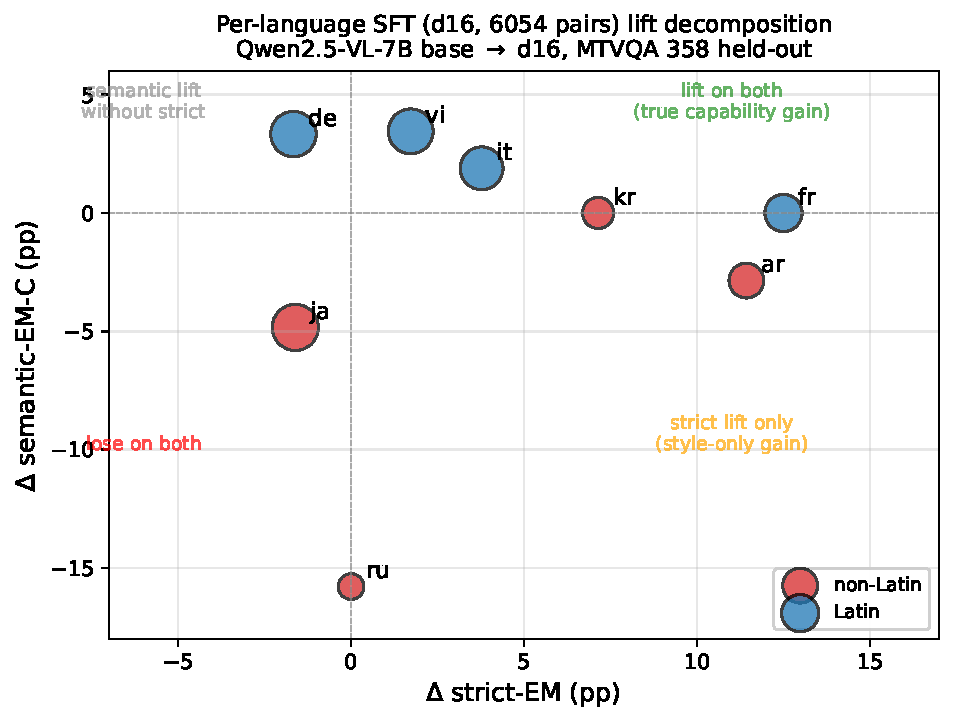
\includegraphics[width=0.95\columnwidth]{figures/fig_sft_anticorrelation.pdf}
\caption{Per-language $\Delta$strict-EM vs $\Delta$semantic-EM-C under d16 anchor-only SFT (base Qwen2.5-VL-7B $\to$ d16, 358 held-out). Latin scripts (blue) lift both axes or are neutral. Non-Latin scripts (red) cluster in the bottom-right (style lift, semantic damage) and bottom-left (loss on both). Marker area $\propto n$. Thai ($n=3$) excluded.}
\label{fig:anticorrelation}
\end{figure}

\section{XFUND within-CJK and cross-script}
\label{app:xfund}

We replicate the strict-vs-semantic protocol on XFUND \citep{xu2022xfund} across 7 languages, stratified-sampling 200 rows per language ($n=1400$; 1394 cleanly judged after retry-exhaustion drops) from Qwen2.5-VL-7B test predictions and judging with the same Gemini-Flash prompt. Table~\ref{tab:xfund-cjk} reports the within-CJK Japanese-vs-Chinese gap.

\begin{table}[t]
\centering
\small
\begin{tabular}{lrrrr}
\toprule
& ja & zh & zh$-$ja gap & artifact \\
\midrule
strict-EM       & 13.0\% & 42.6\% & $+29.6$ pp & --- \\
semantic-EM-C   & 30.0\% & 55.9\% & $+25.9$ pp & 12.4\% \\
semantic-EM-C+P & 46.5\% & 66.7\% & $+20.2$ pp & 31.8\% \\
\bottomrule
\end{tabular}
\caption{XFUND within-CJK Japanese vs Chinese gap, base Qwen2.5-VL-7B over $n=200$ ja + $n=195$ zh judged rows. The strict-EM gap of $+29.6$ pp shrinks only to $+25.9$ pp under semantic-CORRECT: artifact share $12\%$. The within-CJK gap is \emph{not} a measurement artifact.}
\label{tab:xfund-cjk}
\end{table}

\paragraph{Cross-script Latin vs CJK on XFUND.}
On the same 1394-row sample the script-level Latin/CJK strict-EM gap is small ($+1.6$ pp) and shrinks further under semantic-EM ($+1.1$ pp, artifact share $35\%$). XFUND's annotation conventions for Latin scripts produce gold strings closer in surface form to model outputs than MTVQA's; the cross-script gap on XFUND is therefore both smaller and less artifact-laden than on MTVQA, while the within-CJK gap is large and survives. The two datasets carry complementary signal, and the semantic-EM decomposition makes the complementarity visible.

\section{Worked example: applying R1--R9}
\label{app:protocol-example}

Consider a hypothetical method paper reporting ``$+5.0$ pp Arabic strict-EM lift on MTVQA via decoding-side OCR injection.'' Under current convention this is a publishable single-number claim. Under the protocol of \S\ref{sec:protocol}, the same paper must additionally report: Arabic semantic-EM-C before and after with CIs (R1, R2); cross-judge or human agreement on a $\geq 50$-row sample (R4); retry-exhaustion accounting for the judge run (R5); output-style penalty before and after the intervention (R6); per-language $\Delta$ for every other language in the evaluation, not just Arabic (R8); and public release of judge tuples for third-party re-judging (R9). If post-intervention Arabic semantic-EM-C is unchanged, the lift is normalisation, not capability. If post-intervention Arabic semantic-EM-C \emph{decreases}, the lift is capability damage masked by style alignment (the pattern observed in our d16 SFT decomposition; Table~\ref{tab:sft-perlang}). If both lift, the intervention is real. The protocol does not adjudicate the method's worth --- it makes the answer to ``did this help or hurt?'' visible to the reader.


\end{document}
